\documentclass[conference]{llncs}
\usepackage{amssymb}
\usepackage{amsmath}
\usepackage{url}
\usepackage{hyperref}
\usepackage{amsopn}
\usepackage{listings}
\usepackage{graphicx}
\usepackage{etoolbox}
\usepackage{booktabs}
\usepackage{multirow}
\usepackage[noend]{algpseudocode}
\usepackage[font=footnotesize]{subfig}

\usepackage{tablefootnote}
\usepackage{bigstrut}

\usepackage{geometry}
\geometry{
  a4paper,         % or letterpaper
  textwidth=15cm,  % llncs has 12.2cm
  textheight=24cm, % llncs has 19.3cm
  hratio=1:1,      % horizontally centered
  vratio=2:3,      % not vertically centered
}


\newcommand{\union}{\cup}
\newcommand{\intersects}{\cap}
\newcommand{\refdefinition}[1]{Def.~\ref{#1}}
\newcommand{\reffigure}[1]{Fig.~\ref{#1}}
\newcommand{\refsection}[1]{\S~\ref{#1}}
\newcommand{\reflemma}[1]{Lemma.~\ref{#1}}
\newcommand{\refexample}[1]{Example.~\ref{#1}}
\newcommand{\reftable}[1]{Table.~\ref{#1}}
\newcommand{\reftheorem}[1]{Theorem.~\ref{#1}}
\newcommand{\refequation}[1]{Equation.~\ref{#1}}
\newcommand{\refappendix}[1]{Appendix}
\newcommand{\refcorollary}[1]{Corollary.~\ref{#1}}
\newcommand{\zap}[1]{ }

\setcounter{secnumdepth}{3}

\makeatletter 

\renewcommand\subsubsection{\@startsection{subsubsection}{3}{0mm} 
{-\baselineskip} 
{1\baselineskip} 
{\normalfont\normalsize\bfseries} 
}
\makeatother 


\subtitle{Towards Big Active Data Management}
\title{Research Proposal}
\author{Chen Luo}
\institute{}

\begin{document}
\maketitle

\section{Introduction}
A large volume of data is being generated on a continuous basis, such as tweets, clickstreams, and sensor output.
In the meanwhile, with the advancement of data analytics and cloud computing techniques, organizations today are collecting and analyzing these continuous data for various purposes.
For example, a retail company may analyze posted tweets to discover users' interests.
An advertisement company might learn users' preferences from clickstreams.
Unfortunately, today's data management systems provide little support for collecting and loading continuous data, which is the first step for enabling data analysis.


Thus, engineers often have to manually implement external functionalities to collect and load continuous data into data management systems.
However, this ad-hoc solution suffers from several drawbacks in practice.
First, it is often challenging to implement scalable external functionalities to collect and load fast-generating continuous data (scalability).
Moreover, these functionalities usually involve an extra copy of data (space-inefficiency), and fail to directly manipulate the underling storage of the data management systems for efficient loading (time-inefficiency).
Finally, re-engineering efforts are required to implement these functionalities repeatedly under different scenarios. 
For these reasons, it is ideal for today's data management systems to provide native support for collecting and loading continuous data, or, in other words, \emph{data ingestion}.

In this research proposal, we present the data ingestion component inside today's data management systems for managing active data.
In this active setting, data are generated, collected, and loaded on a continuous basis.
As in~\cite{ingestion2015}, we use the term \emph{data feed} to refer to a flow of data from an external source.
Thus, the data ingestion component is essentially responsible for continuously fetching data from external sources, transforming data as required, and then storing them persistently, according to the defined data feeds.
However, engineering a practical data ingestion component is highly nontrivial, and at least the following challenges need to be addressed.
\begin{itemize}
\item Generality: Serving for a general purpose, the component should be able to work with various data sources and applications.
Flexible and fine-grained configurations are also necessary to satisfy diverse application requirements.

\item Efficiency \& Scalability: In order to ingest the large volume of fast-generating data, the component should be efficient and scalable enough.
It is also desirable for the component to directly manipulate the underling storage for efficient data loading, instead of naively calling the insert command provided by data management systems.

\item Elasticity: The component is expected to run continuously with multiple fluctuating feeds. Thus, it is ideal for the component to offer elasticity by being able to dynamically scale in/out resources based on the workloads.

\item Fault-Tolerance: Running on commodity servers, the component should provide fault-tolerance mechanisms to handle software/hardware failures. Several fault-tolerance mechanisms with varying data loss guarantees should be designed to satisfy different application requirements.

\end{itemize}
The remaining of the proposal is organized as follows. \refsection{sec:related-works} briefly reviews related works.
\refsection{sec:research-design} presents a preliminary architectural design of the component.
Finally, \refsection{sec:conclusion} concludes the proposal.

\section{Related Works}
\label{sec:related-works}
Most state-of-the-art big data systems, including MapReduce~\cite{mapreduce2008}, Spark~\cite{spark2012}, and HadoopDB~\cite{hadoopdb2009} etc., provide no direct support for ingesting continuous data, but rather simply assume the data are in place.
One exception is AsterixDB~\cite{ingestion2015}, which is equipped with the first data ingestion functionality.
However, the data ingestion functionality provided by AsterixDB is still at a preliminary stage and misses many features discussed in the proposal (\refsection{sec:research-design}), such as declarative feed definition, fine-grained feed configuration, lazy transformation, and storage-aware data insertion.
It is expected that the proposed component would significantly enrich the data ingestion functionality for today's big data systems.

Stream data processing systems~\cite{spade2008,s42010,spark-stream2012} share some similarity with the proposed data ingestion component in that both consider continuous data. However, the major difference is that stream data processing systems only process data without storing them. The drawbacks of implementing data ingestion functionalities with these systems have been discussed in the previous section.
Moreover, \cite{ingestion2015} further shows combining stream data processing systems, e.g., Storm, with data management systems, e.g., MongoDB, for the data ingestion purpose may subject to suboptimal performance.
But still, many ideas and techniques in stream data processing, e.g., architectural design, query processing, and fault tolerance, could be borrowed for the design of our data ingestion component.

\section{Research Design}
\label{sec:research-design}
In this section, we present an architectural design of the proposed data ingestion component.
Although the component is to be implemented inside a specific data management system, we do not limit our discussion to any specific system in order to be more general.
The architecture of the proposed component is shown in \reffigure{fig:architecture}.
The component mainly consists of two modules, i.e., \emph{feed definition} as a user interface and \emph{feed runtime} for executing and managing data feeds.
%In the following discussion, we assume a semi-structured data model, where a schema is available in advance, but the records in the table are allowed to have extra fields.

\begin{figure}[t]
\centering
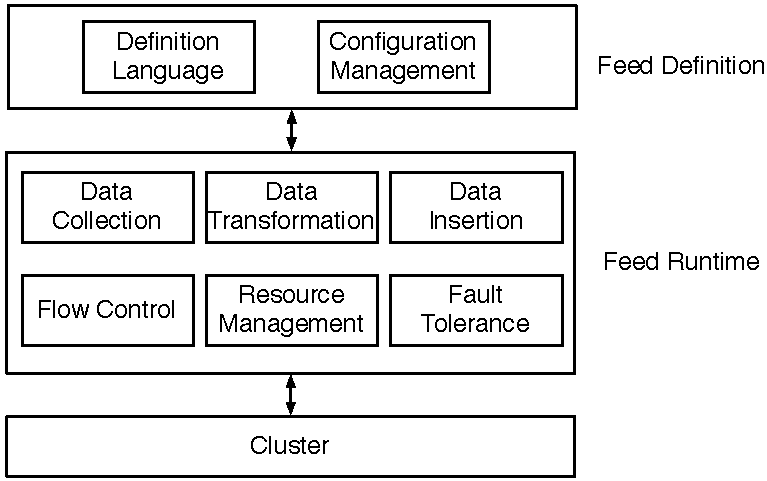
\includegraphics[width=0.45\linewidth]{architecture.pdf}
\caption{Architectural Design of the Proposed Component}
\label{fig:architecture}
\end{figure}

\subsection{Feed Definition}
The feed definition module provides a SQL-like declarative language for the user to define data feeds.
A data feed contains three parts: a data source, data transformations and a target.
A data source can be either a \emph{feed adapter} which parses raw byte streams into records, or an existing data feed.
Data transformations allow the user to transform the original records, including projection, window aggregation, filtering, and sampling etc.
Finally, a target specifies where the data should be stored, such as a table or a file.

In addition to the definition language, the module also allows the user to configure data feeds.
Example configurations include priority, fault tolerance, and desired degree of parallelism etc.
Some of the configurations are necessarily at a fine-grained level, i.e., record level, since the records in a feed could have different requirements.
For example, the tweets on some hot topics would be more valuable than other tweets, and thus require higher priorities.

\subsection{Feed Runtime}
With the defined data feeds, the feed runtime module then executes them to ingest data continuously.
The feed runtime module also contains some other submodules responsible for flow control, fault tolerance, and resource management.
Note that although these submodules are depicted independently in \reffigure{fig:architecture} for ease of illustration, they are tightly integrated with the feed execution submodules during the data ingestion process.

\subsubsection{Feed Execution}
The defined data feeds essentially form a (logical) directed acyclic graph (DAG), where the source nodes are data sources, the internal nodes are transformations, and the sink nodes are persistent storages.
To execute the feeds, the component first optimizes the DAG, and then compiles the optimized DAG into an execution plan, whose stages are discussed below.
Note that data feeds may be registered/unregistered dynamically, which requires the component being able to modify the execution plan on the fly.

\textbf{Data Collection.}
In the first stage of the execution plan, the component continuously fetches data from data sources with feed adapters.
The fetched data are optionally replicated for fault tolerance, and are then passed to the next stage for transformation.

\textbf{Data Transformation.}
With the fetched data, the component then transforms them as specified by the user.
As mentioned before, these transformations include projection, window aggregation, filtering, and sampling etc.
Note that when a data feed is used to define other feeds, the records might have to be replicated multiple times.
%To avoid replicating records multiple times when a feed is used to define other feeds, the component should adopt a lazy transformation strategy.
A lazy transformation strategy should thus be employed for the throughput consideration.
Briefly, instead of replicating and transforming the data in place, the component could first store the necessary metadata, e.g., the source feed and transformations, and populate the dataset afterwards.

\textbf{Data Insertion.}
As the final step, the component stores the transformed data to the target storage.
Instead of simply calling the insert command, which may incur unnecessary performance degradation, the component should directly manipulate the underling storage and indexes.
Moreover, performance models for different storages and indexes should be developed for the component to choose the optimal data insertion algorithm and the corresponding parameters.
%For the performance consideration, the component should directly manipulate the underling data storage and indexes, instead of simply calling the insert command provided by the system.
%Specific batch insertion algorithms and performance models for different data storages and indexes should also be developed.

\subsubsection{Other Submodules}
After introducing the feed execution submodules, we now focus on other submodules responsible for the non-functional requirements of the data ingestion component.

\textbf{Flow Control.}
In practice, data often arrive at a fluctuating rate.
For example, a large volume of tweets could be posted abruptly in case of some emergent event.
Thus, proper flow control mechanisms should be designed to handle abrupt data arrivals, such as data spilling and priority-based data dropping etc., to ensure the data are properly ingested and the fluctuating feed would not seriously affect the execution of other feeds.

\textbf{Resource Management.}
Since the component is expected to run continuously with fluctuating feeds, it is ideal for the component to elastically manage cluster resources, which is achieved in two folds.
On one hand, on top of the resource management functionality offered by the data management system, the component should be able to automatically request and return resources based on the active data feeds.
On the other hand, the component should also dynamically allocate the requested resources to data feeds according to their workloads and configurations.

\textbf{Fault Tolerance.}
Running on commodity servers, the component should provide fault tolerance mechanisms to handle hardware/software failures.
Since fault tolerance may incur performance degradation, multiple fault tolerance mechanisms with varying data loss guarantees should be designed to fit the requirements of different data feeds while minimizing performance penalties.
For example, data loss is acceptable for clickstreams, but is not for online transactions.
Thus, a weaker fault tolerance mechanism for clickstreams could be employed for better performance.

\section{Conclusion}
\label{sec:conclusion}
In this proposal, we outline the necessity and challenges of the data ingestion component for today's big data systems.
We further propose a preliminary architectural design of the component to address these challenges.
In the future, a lot of efforts are required to further refine and implement the component, including feed processing algorithms, flow control strategies, resource allocation models, and fault tolerance mechanisms etc.
Moreover, extensive experiments need to be performed to evaluate the component, from efficiency, scalability, elasticity to usability and applicability.
Finally, we hope the data ingestion component discussed in this proposal could be an important step for today's big data systems towards managing big active data.

\bibliographystyle{unsrt}
\bibliography{paper.bib}

\end{document}